\documentclass[letterpaper]{article} 
\usepackage[left = 0.5in, right = 0.5in, top = 0.9in, bottom = 0.9in]{geometry}
\usepackage{enumitem}
\usepackage{multicol}
\usepackage[spanish]{babel}
\usepackage[utf8]{inputenc}

\usepackage{amsmath,amssymb,amsthm}
\usepackage{tikz-cd}
\usepackage{mathrsfs}
\usepackage[bbgreekl]{mathbbol}
\usepackage{dsfont}
\usepackage{graphicx}
\graphicspath{{img/}}

\newcommand{\op}{\operatorname}
\newcommand{\Op}{^{\op{op}}}
\newcommand{\scc}{\mathscr C}
\newcommand{\scd}{\mathscr D}
\newcommand{\sce}{\mathscr E}
\newcommand{\sci}{\mathscr I}
\newcommand{\scj}{\mathscr J}
\newcommand{\scx}{\mathscr X}
\newcommand{\var}{\mathrm{Var}}
\newcommand{\Id}{\operatorname{Id}}
\newcommand{\N}{\mathbb N}
\newcommand{\Z}{\mathbb Z}
\newcommand{\Q}{\mathbb{Q}}
\newcommand{\I}{\mathbb{I}}
\newcommand{\R}{\mathbb{R}}
\newcommand{\C}{\mathbb{C}}
\newcommand{\F}{\mathcal{F}}
\newcommand{\G}{\mathcal{G}}
\newcommand{\B}{\mathcal{B}}
\newcommand{\abs}[1]{\left\lvert #1 \right\rvert}
\newcommand{\inv}{^{-1}}
\renewcommand{\to}{\rightarrow}
\newcommand{\ent}{\Longrightarrow}
\newcommand{\E}{\mathbb{E}}
\renewcommand{\P}{\mathbb{P}}
\newcommand{\1}{\mathds{1}}
\renewcommand{\qedsymbol}{$\blacksquare$}

\theoremstyle{definition}
\newtheorem{dfn}{Definición}
\theoremstyle{definition}
\newtheorem{teo}{Teorema}
\theoremstyle{definition}
\newtheorem{cor}{Corolario}
\theoremstyle{definition}
\newtheorem{prop}{Proposición}
\theoremstyle{definition}
\newtheorem{obs}{Observación}


\title{\textbf{Cómputo Científico\\
Tarea 6\\
}}
\author{Iván Irving Rosas Domínguez}
\date{\today}

\DeclareSymbolFontAlphabet{\mathbbm}{bbold}
\DeclareSymbolFontAlphabet{\mathbb}{AMSb}
\DeclareMathSymbol\bbDelta  \mathord{bbold}{"01}

\begin{document}
\maketitle

%\begin{abstract}
%\end{abstract}
\begin{enumerate}
    \item[\textbf{1.}] Simular $n=5$ y $n=40$ v.a. Bernoulli $Be(1/3)$; sea $r$ el número 
    de éxitos en cada caso.\\

    \textbf{Solución:} El ejercicio se encuentra en el script 'Cómputo Tarea 6' en la primera parte del enunciado. En él, se simulan las 
    variables Bernoulli de parámetro $p=1/3$ y se guardan en los vectores $n5$ y $n40$ para las muestras de 5 y 40 respectivamente,
    mientras que en $r5$ y $r40$ se guarda el número de éxitos de las muestras respectivas.\\

    Con motivos de reproducción de resultados, se coloca una semilla con valor $seed=10$. Con ese valor, la muestra de 5 bernoulli's tiene 2 éxitos mientras que la muestra de
    40 bernoulli's tiene 13 éxitos.\\

    \item[\textbf{2.}] Implementar el algoritmo Metrópolis-Hastings para simular de 
    la posterior 
    \[
    f(p|\bar{x})\propto p^r(1-p)^{n-r}\cos(\pi p)\1_{[0,\frac{1}{2}]}(p),    
    \]
    con los dos casos de $n$ y $r$ de arriba. Para ello poner la propuesta $(p'|p)=p'\sim Beta(r+1,n-r+1)$
    y la distribución inicial de la cadena $\mu\sim U(0,\frac{1}{2})$.
    \newline

    \textbf{Solución:} esta parte del ejercicio se encuentra en la segunda parte del script mencionado antes. En él, se construyen primero 
    tres funciones: $post$, la cual permite evaluar la función posteriori del ejercicio. Esta función tiene tres parámetros, dependiendo 
    justamente del número de ensayos $n$, de éxitos $r$ y del punto a evaluar.\\

    Creamos también la función $mh\_quotient$, la cual calcula el cociente de Metrópolis-Hastings, dado por 
    \[
    \frac{f(y)}{f(x)}\frac{q(x|y)}{q(y|x)},    
    \]
    y que, como $q$ la propuesta es independiente del valor en el cual se encuentra la cadena, y 
    tiene distribución $Beta(r+1,n-r+1)$, entonces el cociente anterior está bien definido.
    La función anterior tiene tres parámetros, nuevamente dependiendo del número de ensayos, éxitos y 
    el punto a evaluar.\\

    Finalmente creamos la función $m\_hast\_beta$, que depende de los parámetros $k$, $n$ y $r$, 
    y que calcula $k$ muestras de la cadena de Markov con la que pretendemos alcanzar la distribución $f$.\\

    Descrito lo anterior, se procede a estudiar los dos ejemplos:

    \begin{itemize}
        \item[\textbf{Ej.1: n=5.}] Como dijimos, el valor de la semilla $seed=10$ arroja un valor de $r=2$ para este caso. 
        Se ejecuta el algoritmo de Metrópolis-Hastings con 1 millón de iteraciones.\\

        Como primer paso, se calcula el logaritmo de la función objetivo evaluada en las muestras. El resultado se ve en la 
        figura 1.

        \begin{figure}[h!]
            \centering
            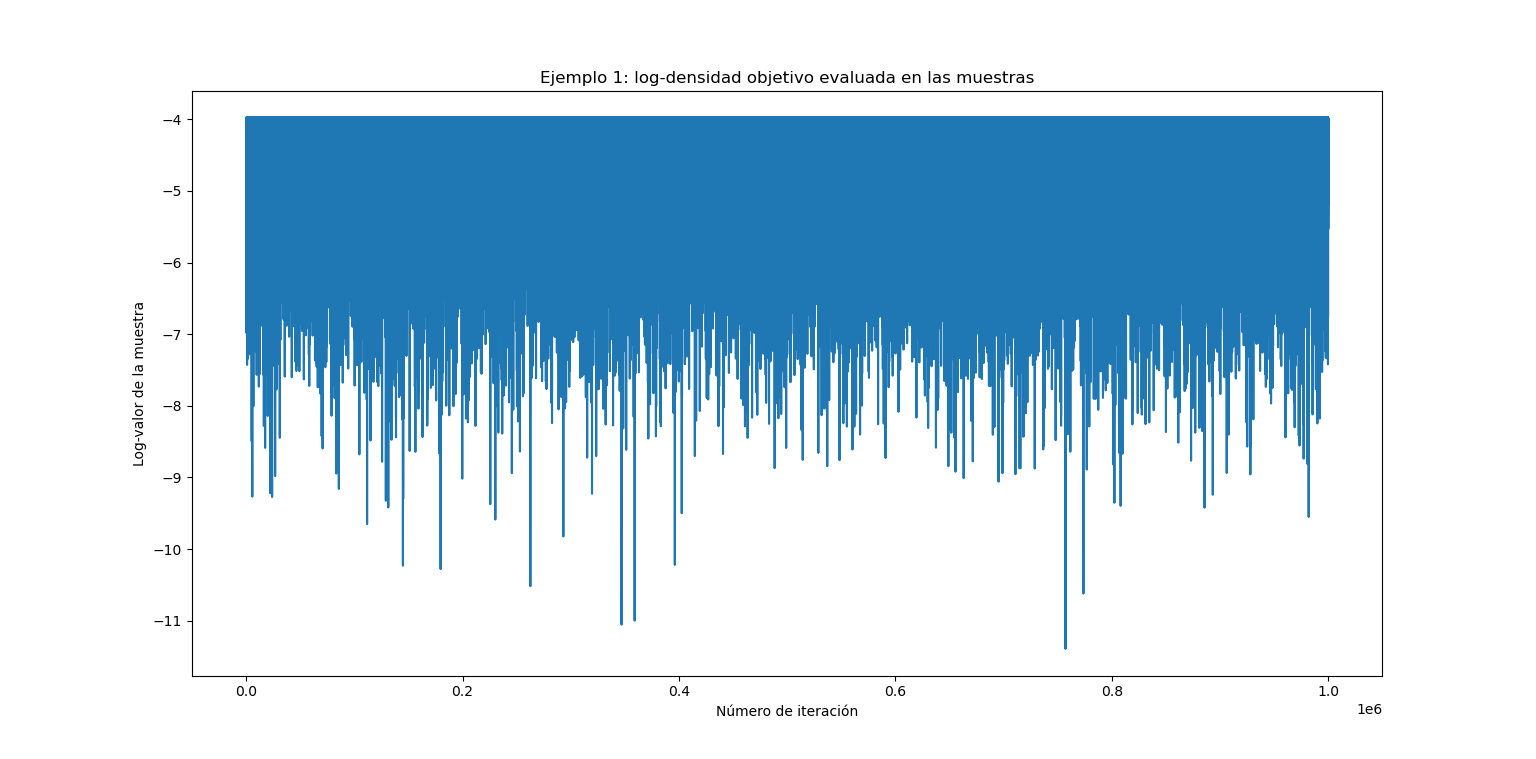
\includegraphics[width=\linewidth]{1.png}
            \caption{Ejemplo 1. $n$=5. La log-densidad evaluada en las muestras. No se nota un patrón anormal inicial.}
        \end{figure} 

        Dado el tamaño tan grande de la muestra, y a que ciertamente de la gráfica no es visible un patrón inicial anormal, 
        decidimos tomar un burn-in de tamaño 50 000. Esto nos deja con un margen adecuado para revisar el histograma de la muestra.
        \newline

        Utilizando Wolfram-Alpha, calculamos la constante de normalización de la densidad objetivo. En este primer caso, está dada por 
        $C_1\approx 188,04733$. Creando una rejilla para calcular la densidad y contrastarla, y graficando el histograma de esta muestra, 
        obtenemos los resultados de la figura 2.
        \begin{figure}[h!]
            \centering
            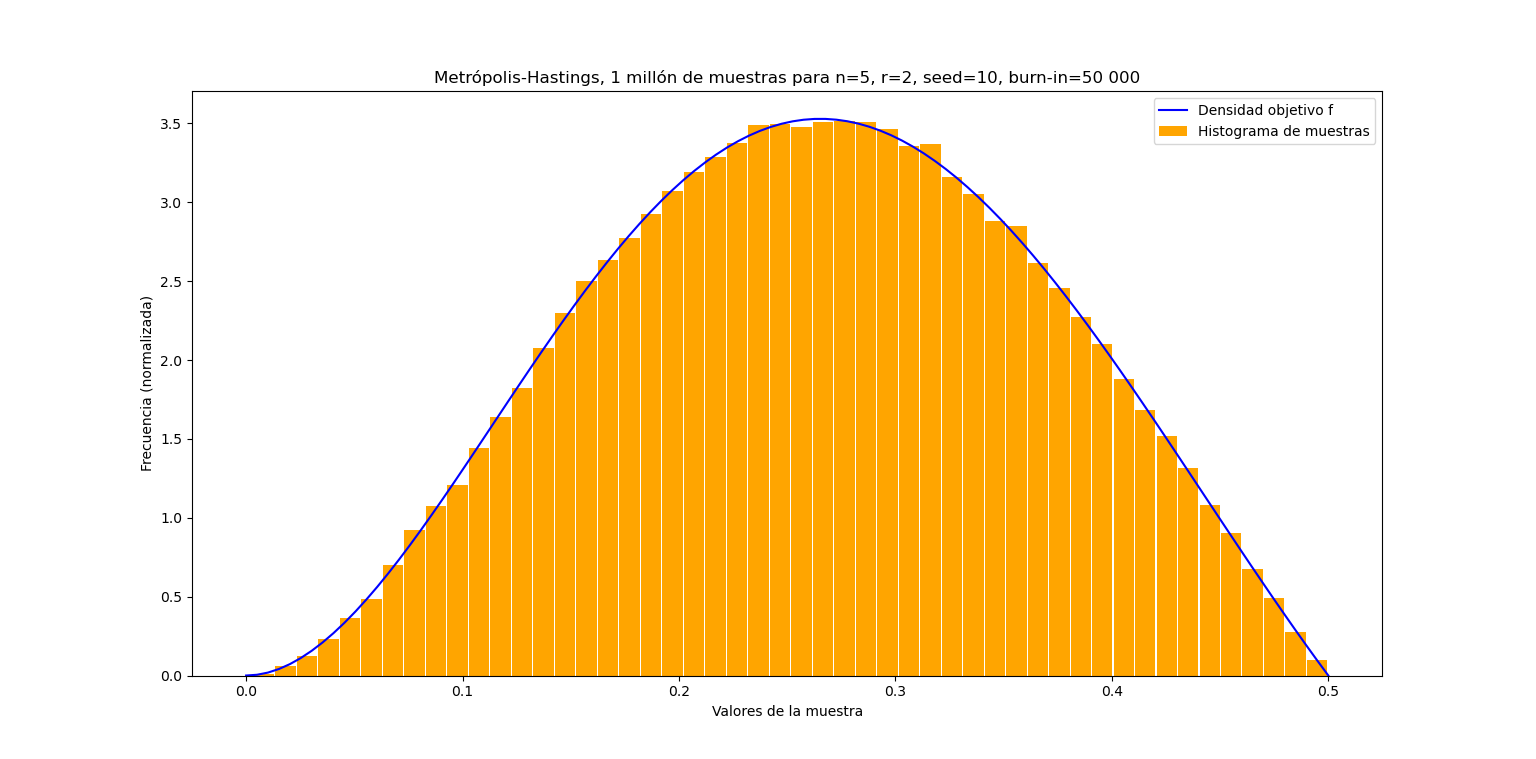
\includegraphics[width=\linewidth]{2.png}
            \caption{Ejemplo 1. $n=5$. Histograma contrastado con la densidad objetivo.}
        \end{figure} 
        Podemos observar de la figura 2 que el ajuste del histograma es bastante bueno, por lo que es confiable utilizar 
        la muestra obtenida como una muestra de la distribución objetivo.\\

        \item[\textbf{Ej.2: n=40.}] El valor de la semilla nos arroja un número de éxitos de $r=13$. Luego, realizando el 
        algoritmo con 1 millón de muestras, y graficando primero la log-densidad objetivo evaluada en el millón de muestras,
        obtenemos los resultados de la figura 3.

        \begin{figure}[h!]
            \centering
            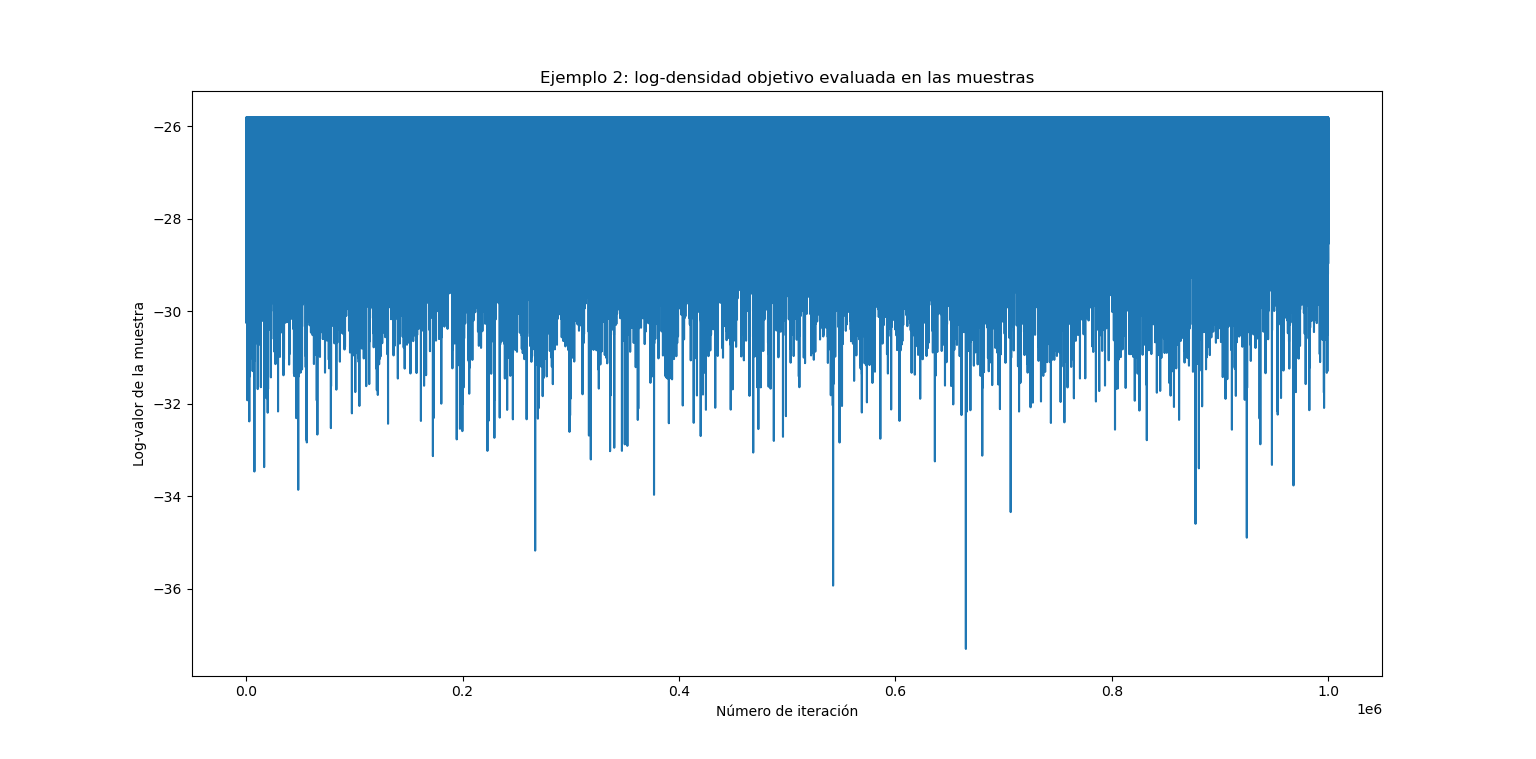
\includegraphics[width=\linewidth]{3.png}
            \caption{Ejemplo 2. $n=40$. La log-densidad evaluada en las muestras. Tampoco se nota un patrón anormal inicial.}
        \end{figure}

        Nuevamente no es perceptible un número en el cual la cadena esté lejos de la distribución objetivo, por lo que 
        aprovechando el tamaño de la muestra, nuevamente tomamos las primeras 50 000 muestras y las desechamos. Calculamos 
        nuevamente la constante de normalización de la función, la cual está dada por $C_2\approx 1009076644417$, y graficando 
        la distribución objetivo versus el histograma de muestras, obtenemos los resultados de la figura 4.

        \begin{figure}[h!]
            \centering
            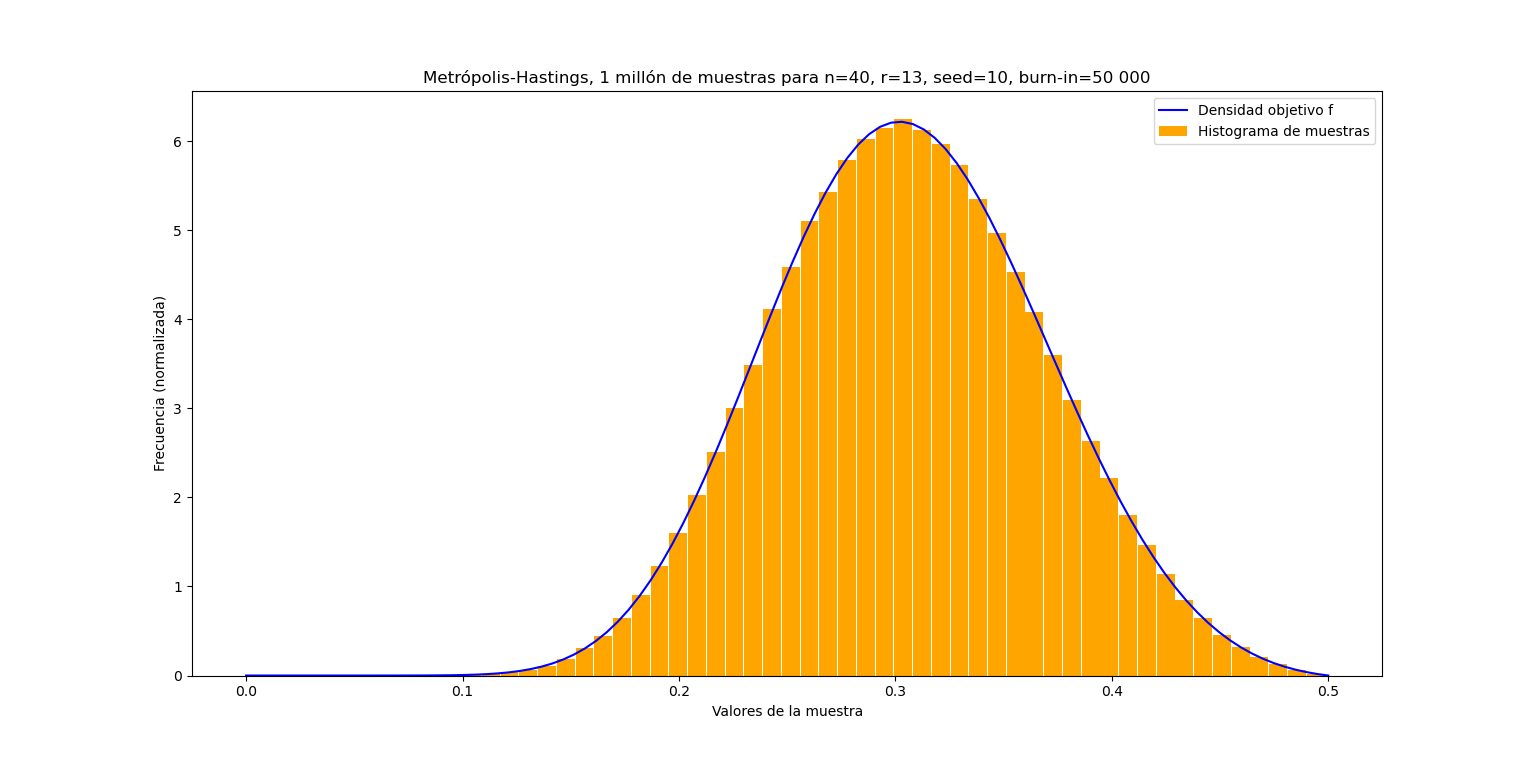
\includegraphics[width=\linewidth]{4.png}
            \caption{Ejemplo 2. $n=40$. Histograma contrastado con la densidad objetivo.}
        \end{figure}

        Nuevamente el ajuste es bastante bueno, por lo que se puede considerar la muestra obtenida como una muestra de la distribución 
        deseada.
    \end{itemize}
    \item[\textbf{3.}] Argumentar por qué la cadena es $f$-irreducible y por qué es ergódica. 
    Implementar el algoritmo con los datos descritos y discutir los resultados.\\

    \textbf{Solución:} aseguramos que la cadena es $f$-irreducible. En efecto. Primero que nada, dado que 
    $f$ visto como una medida en el intervalo $[0,\frac{1}{2}]$ es absolutamente continua con respecto 
    a la medida de Lebesgue, basta ver que para cualquier $B\in \mathcal{B}([0,\tfrac{1}{2}])$ con $\lambda(B)>0$, 
    se tiene que existe un $n\geq1$ tal que $K^{n}(x,A)>0$ para cualquier $x\in [0,\frac{1}{2}]$, donde
    $K$ es el kernel de transición de la cadena.
    \newline

    Notamos entonces que para $A$ como se describió antes, 
    \[
    K(x,A)=\P\left(X^{t+1}\in A|X^{t}=x\right)=\int_A \P\left(X^{t+1}=y | X^{t}=x\right)dy=x|\int_A q(y|x)dy,    
    \]
    pero nuestra propuesta tiene densidad también, y esta densidad es no nula en $\frac{1}{2}$, por 
    lo que esta última integral es estrictamente positiva siempre que $\lambda(A)>0$ la medida de 
    Lebesgue de $A$ sea positiva, lo cual ocurre por hipótesis. Tenemos así que la cadena es $f$-irreducible.
    \newline

    Finalmente, la cadena es ergódica, ya que $K$ es $f$-irreducible y $f$ es una medida estacionaria de probabilidad.
    Además, la cadena es fuertemente aperiódica, ya que por la condición $p(x,y)=\min \left\{1,\frac{f(y)}{f(x)}\frac{q(x|y)}{q(y|x)}\right\}$,
    hay probabilidad positiva de que la cadena se quede en el estado actual, ya que 
    \[
        \frac{f(y)}{f(x)}\frac{q(x|y)}{q(y|x)}\propto y^r(1-y)^{n-r}\cos(\pi y)\cdot x^-r(1-x)^{-n+r}\cos^{-1}(\pi x)\cdot \beta(x) \beta^{-1}(y) 
    \]
    el cociente de Metrópolis Hastings es, para este ejemplo, distinto de cero para cualquier $x\in [0,\frac{1}{2}] \ \ \lambda-$casi seguramente. $\beta(p)$ 
    representa la densidad de una variable aleatoria $\beta$ evaluada en $p$.

    \item[\textbf{4.}] Implementar el algoritmo Metrópolis-Hastings con la posterior de arriba 
    tomando una propuesta diferente.\\

    \textbf{Solución:} Implementamos Metrópolis-Hastings, ahora tomando una propuesta uniforme en $[0,\frac{1}{2}]$. Esta propuesta 
    no toma en cuenta los datos $n$ y $r$, por lo que intuitivamente no será mejor que la propuesta anterior.
    \newline

    Después de implementar los dos ejemplos anteriores modificando adecuadamente las funciones que calculan el cociente de Metrópolis-Hastings 
    y el algoritmo mismo, obtenemos los siguientes resultados:
    \begin{itemize}
        \item[\textbf{Ej.1: n=5.}] Seguimos con semilla $seed=10$, por lo que $r5=2$.\\

        Calculando el logaritmo de la función objetivo, tenemos la figura 5.

        \begin{figure}[h!]
            \centering
            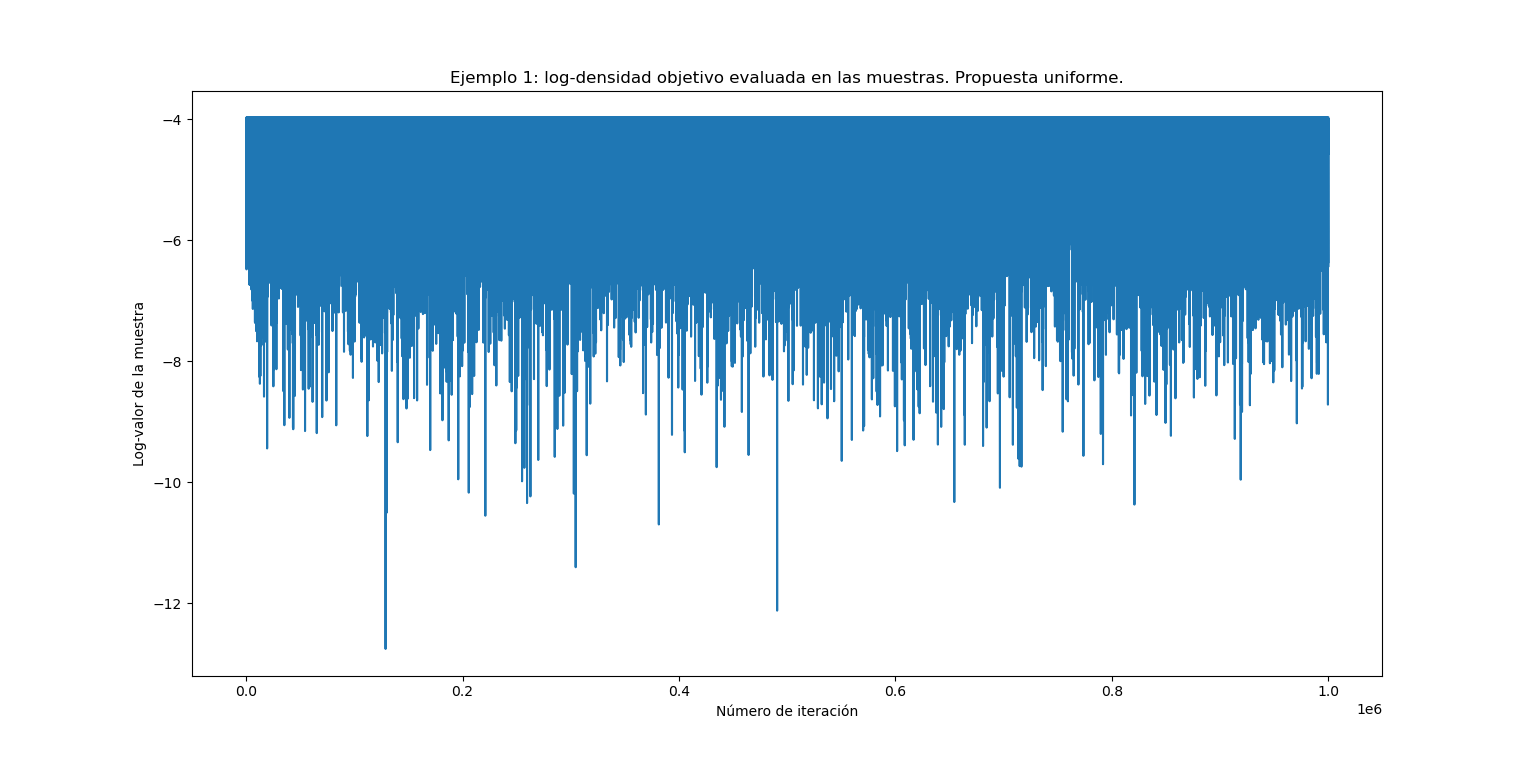
\includegraphics[width=\linewidth]{5.png}
            \caption{Ejemplo 1. $n$=5. La log-densidad evaluada en las muestras., propuesta uniforme. En este nuevo ejemplo no tampoco se aprecia un patrón en las primeras muestras.}
        \end{figure} 

        Nuevamente decidimos tomar un burn-in de tamaño 50 000 gracias a nuestro tamaño de muestra y a que ciertamente no es perceptible algún patrón extraño en 
        la gráfica anterior.
        \newline

        Dado que la densidad objetivo no ha cambiado en este caso, la gráfica de la densidad objetivo es la misma que en el ejemplo 1 del algoritmo anterior.
        Graficando el histograma de esta muestra con esta nueva propuesta, 
        obtenemos los resultados de la figura 6.
        \begin{figure}[h!]
            \centering
            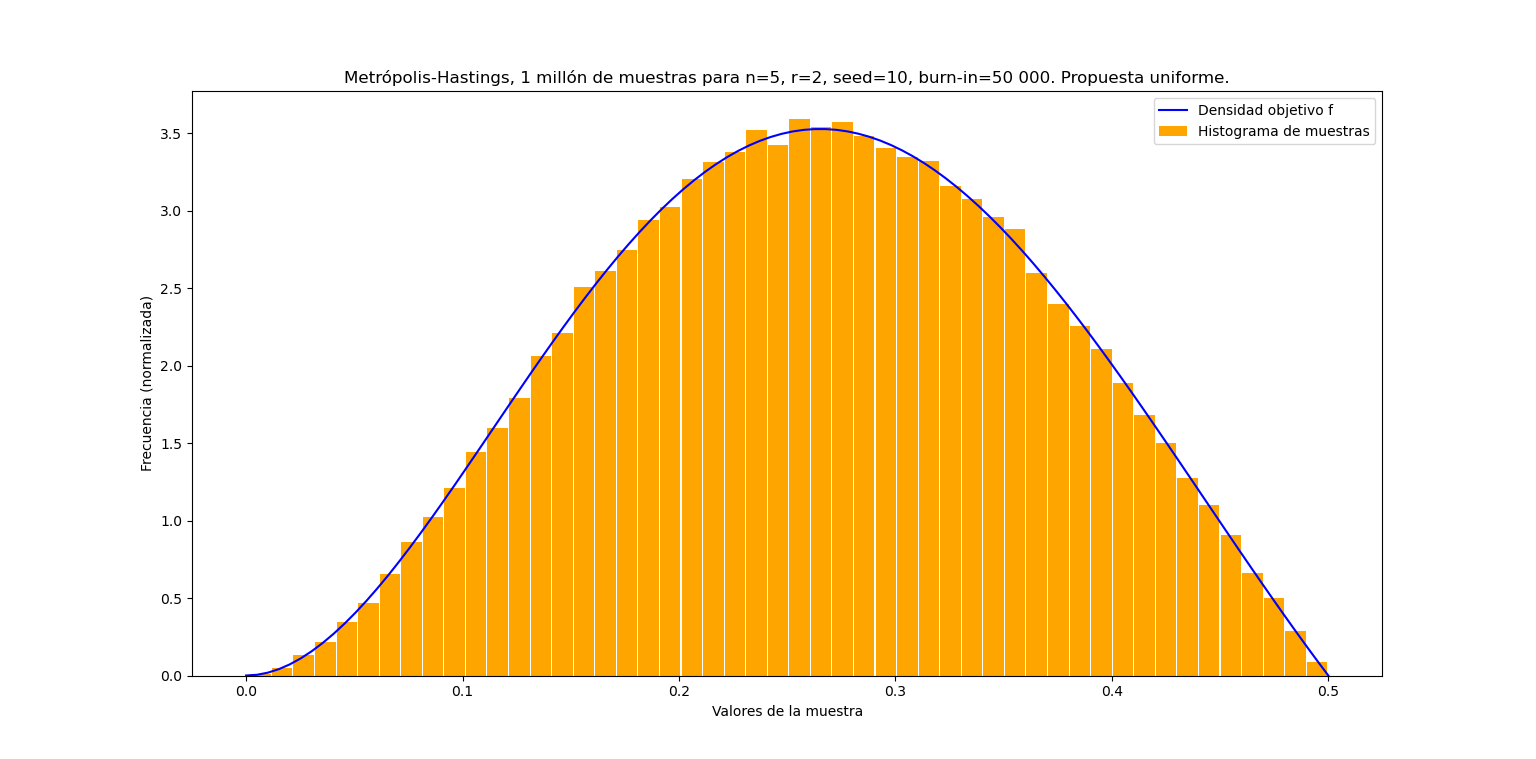
\includegraphics[width=\linewidth]{6.png}
            \caption{Ejemplo 1. $n=5$. Histograma contrastado con la densidad objetivo. Propuesta uniforme.}
        \end{figure} 
        Podemos observar de la figura 6 que el ajuste del histograma también es bastante bueno.\\

        \item[\textbf{Ej.2: n=40.}] Ejecutamos nuevamente 1 millón de muestras. Graficamos la log-densidad evaluada en las muestras y graficamos. Se obtienen 
        los resultados de la figura 7.

        \begin{figure}[h!]
            \centering
            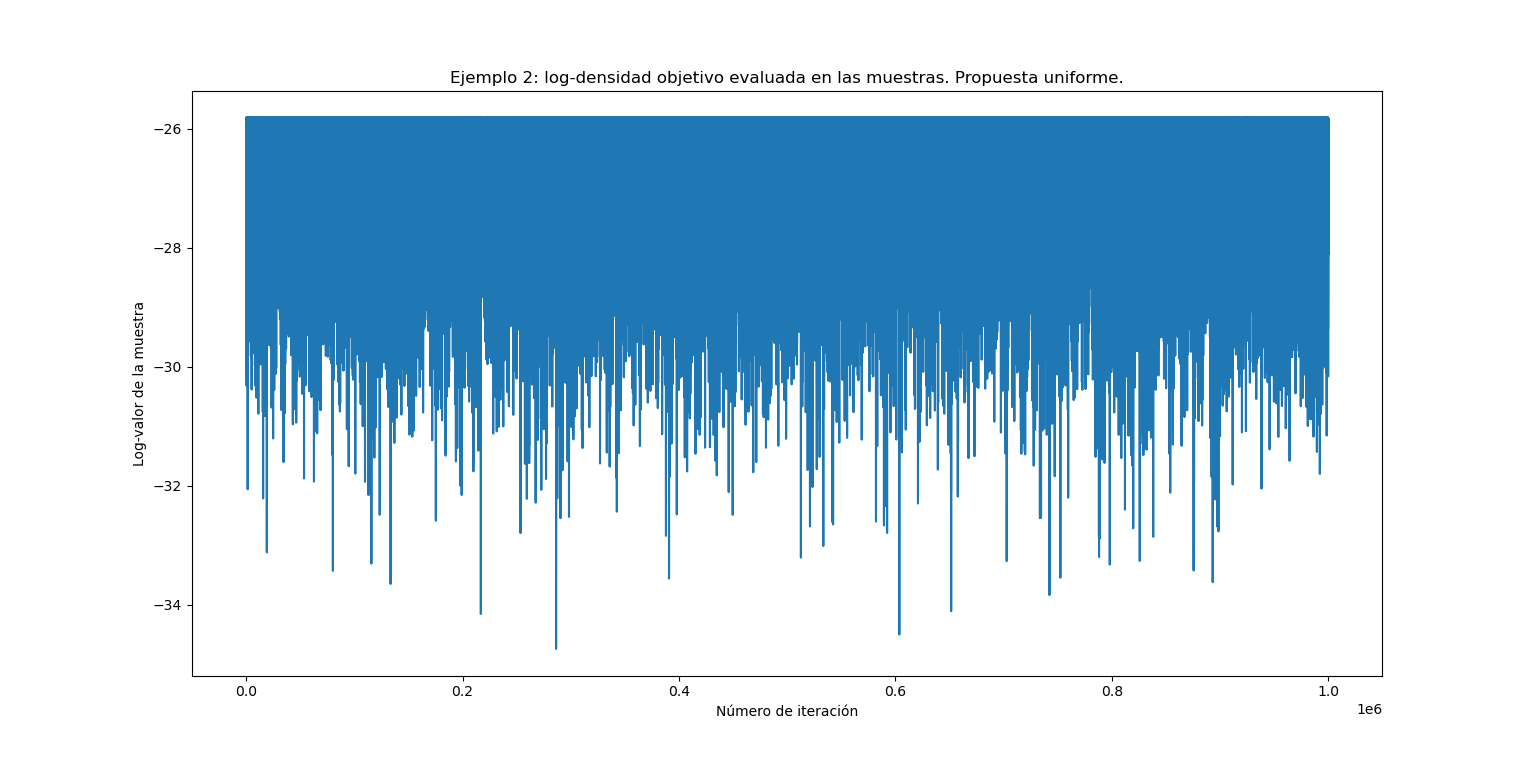
\includegraphics[width=\linewidth]{7.png}
            \caption{Ejemplo 2. $n=40$. La log-densidad evaluada en las muestras. Propuesta uniforme. No se nota un patrón anormal inicial.}
        \end{figure}

        De nueva cuenta no se observa nada extraño al inicio de la gráfica de la log-densidad. Luego, aprovechamos el tamaño de muestra y realizamos un burn-in de 50 000.
        Reutilizamos la gráfica de la densidad pasada y obtenemos los resultados de la figura 8.

        \begin{figure}[h!]
            \centering
            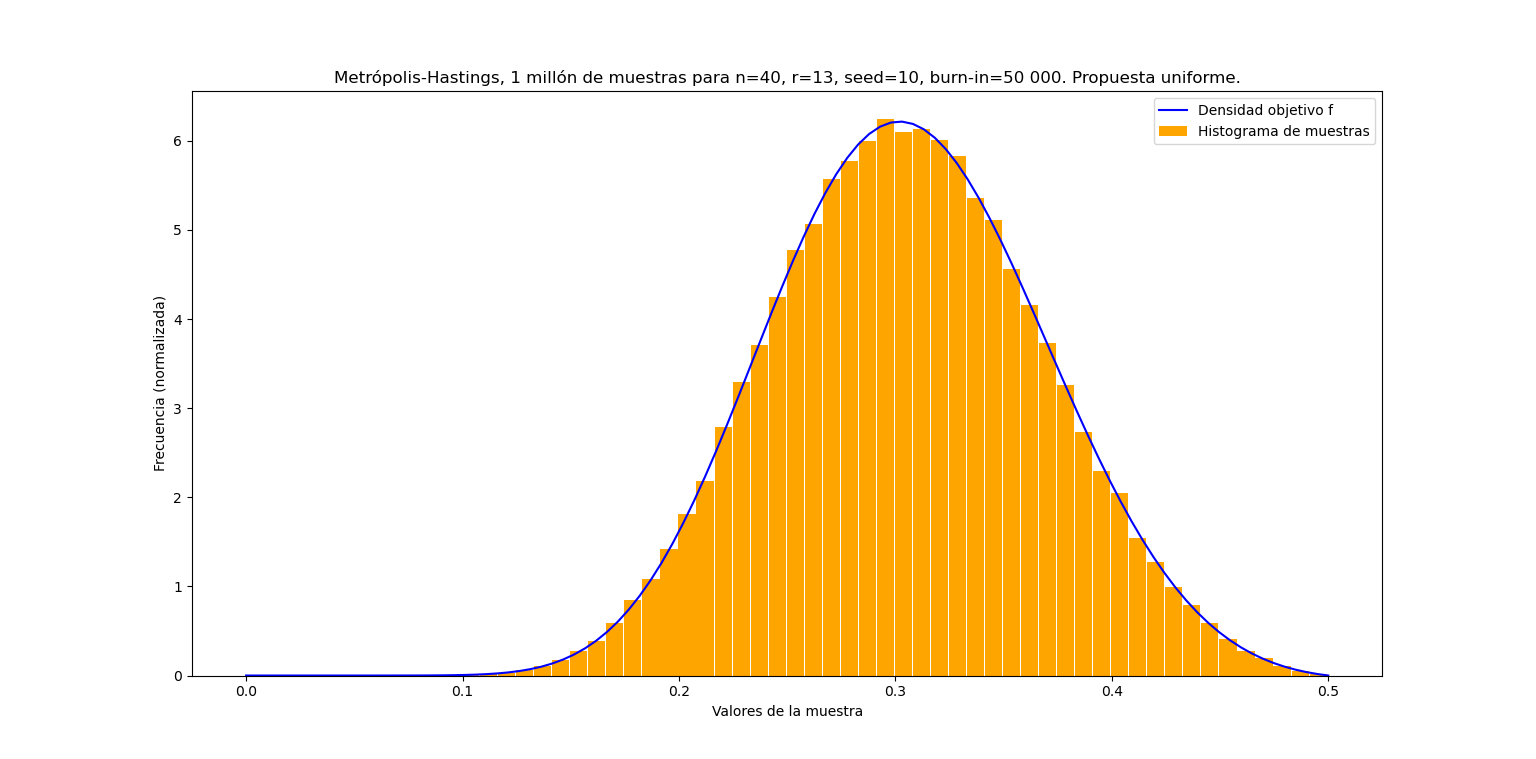
\includegraphics[width=\linewidth]{8.png}
            \caption{Ejemplo 2. $n=40$. Histograma contrastado con la densidad objetivo.}
        \end{figure}

        El ajuste resulta ser bueno.
    \end{itemize}
Finalmente, para completar el ejercicio, realizamos un contraste entre las dos propuestas de transición, en el caso $n=40, r=13$, con muestras más pequeñas.
Ciertamente con 950 000 muestras (quitando el Burn-in) en ambas
resulta un ajuste bueno, sin embargo, si disminuimos el número de muestras e implementamos un Burn-in de solo 20 000, observamos los resultados de las figuras 9 y 10.

\begin{figure}[h!]
    \centering
    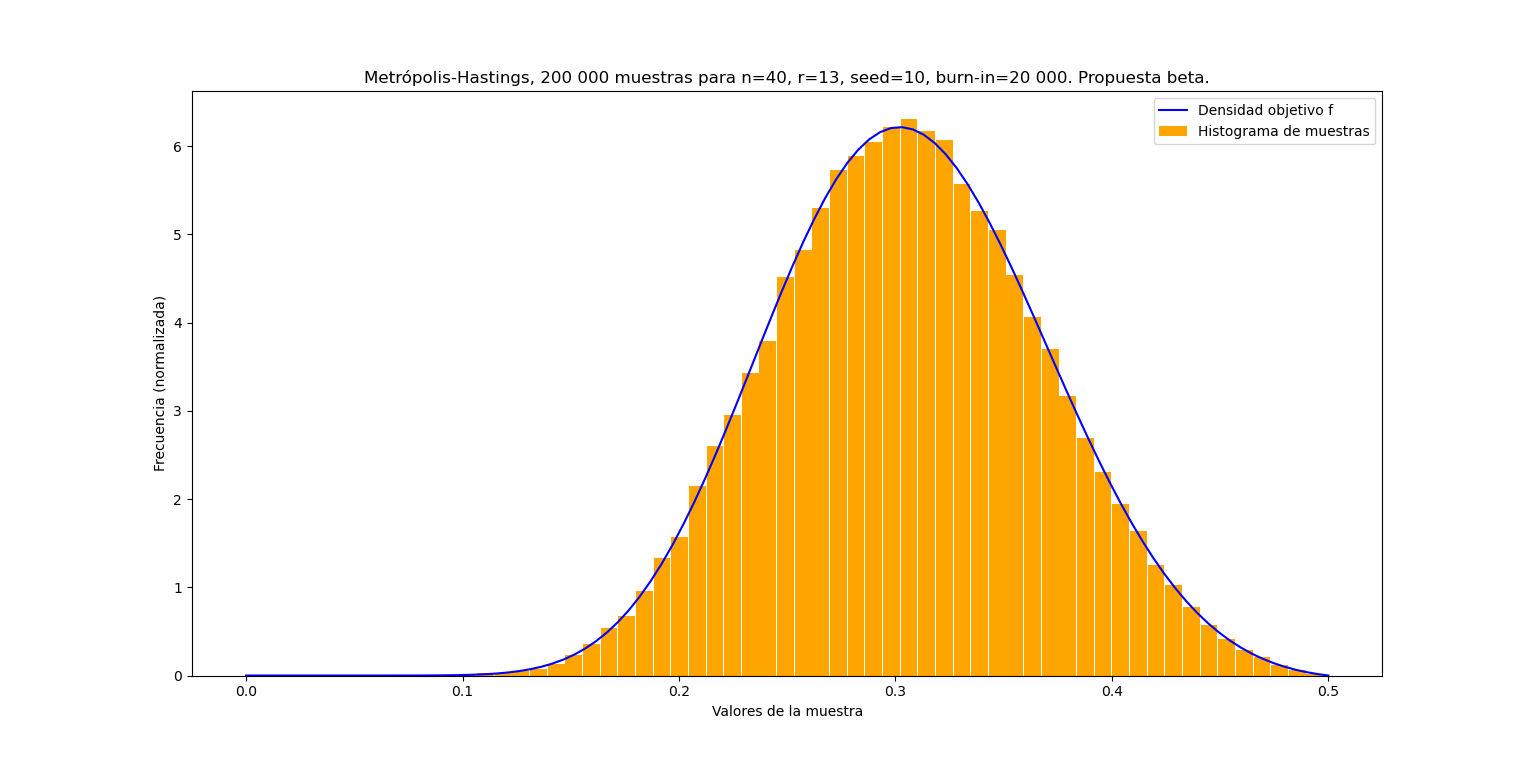
\includegraphics[width=\linewidth]{9.png}
    \caption{Ejemplo 2. $n=40$. Propuesta Beta($r+1,n-r+1$). Histograma contrastado con la densidad objetivo.}
\end{figure}

\begin{figure}[h!]
    \centering
    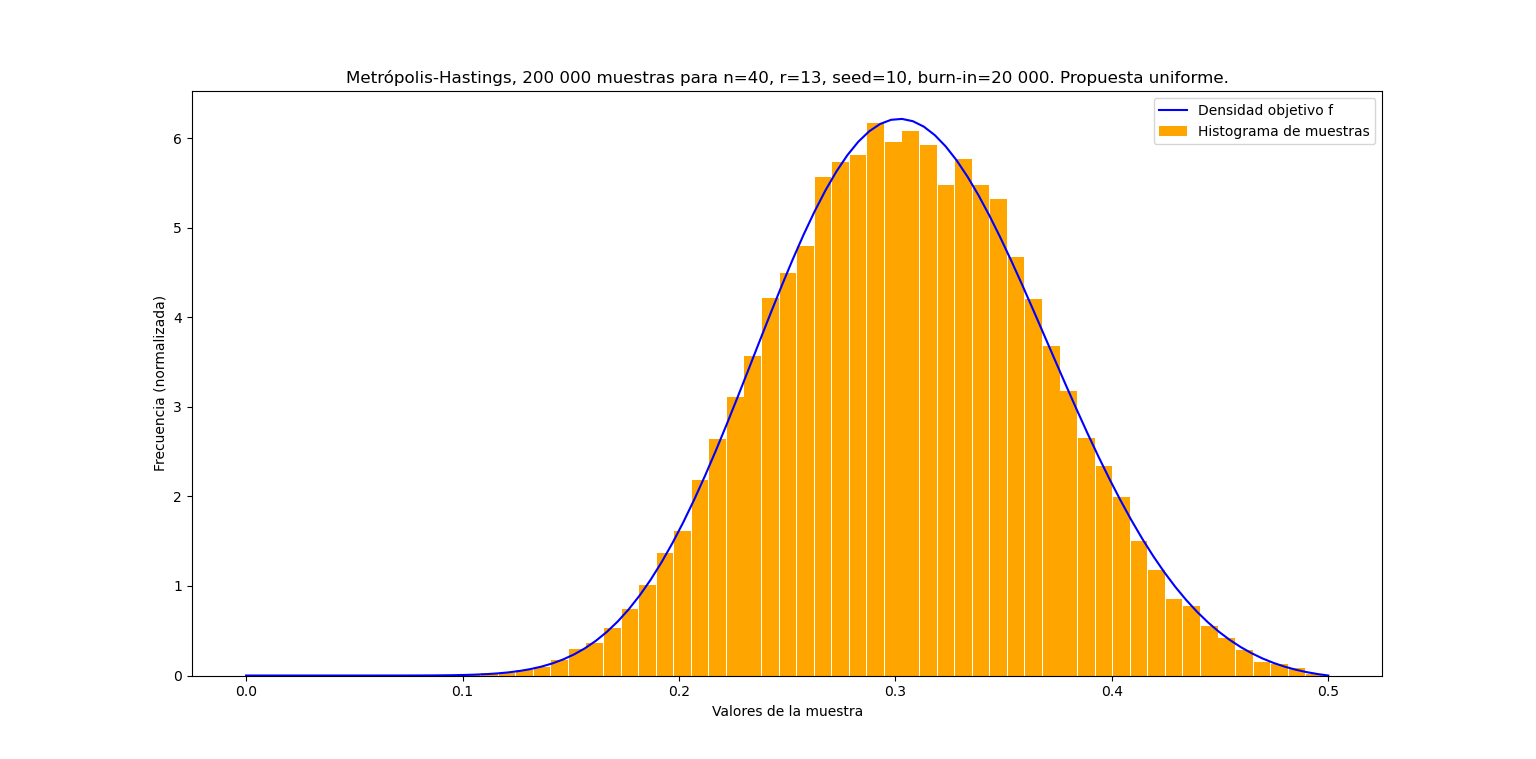
\includegraphics[width=\linewidth]{10.png}
    \caption{Ejemplo 2. $n=40$. Propuesta Uniforme(0,1). Histograma contrastado con la densidad objetivo.}
\end{figure}
Podemos notar un ligero mejor ajuste en la propuesta beta que en la uniforme, por lo que el algoritmo es más eficiente con la primera propuesta 
que con la segunda.
\end{enumerate}
\end{document}